\section{Simple Power Analysis (SPA)}

\begin{frame}
    \frametitle{Simple Power Analysis (SPA)}
    \begin{block}{What is SPA? }
        \begin{itemize}
            \item Attack technique based on the \textbf{direct visual interpretation} of power consumption traces from a cryptographic device.
            \item SPA attacks exploit key-dependent patterns within a trace
            \item They use only one trace (or very few traces)
            \item This was one of the first power analysis techniques to be publicly described.
        \end{itemize}
    \end{block}
\end{frame}

\begin{frame}
    \begin{figure}
        \centering
        \begin{minipage}{0.48\textwidth}
            \centering
            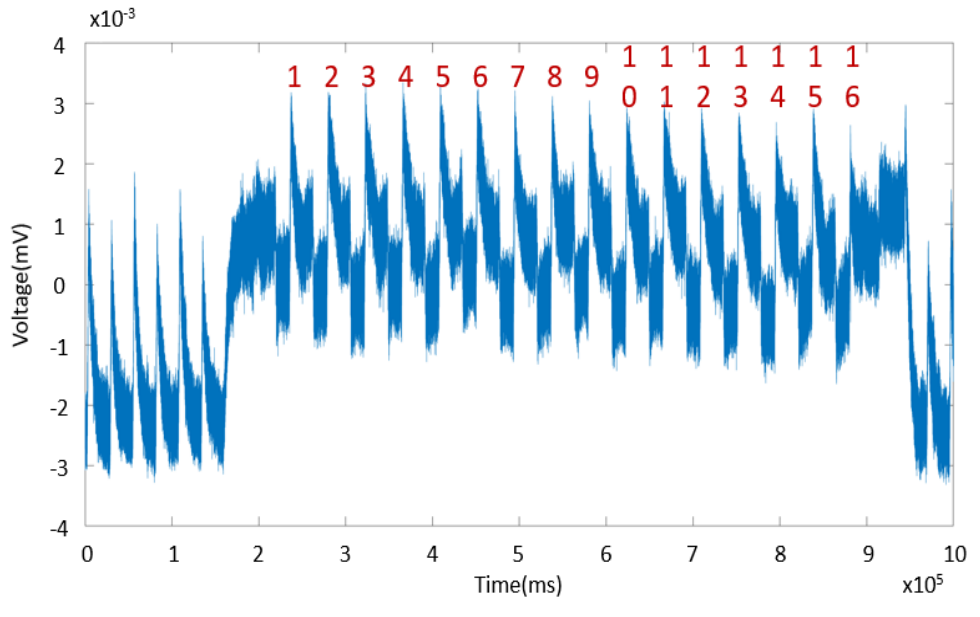
\includegraphics[width=\linewidth]{main thing/Pictures/DES_SPA_trace.png}
            \captionof{figure}{\small An SPA trace showing the 16 rounds of a DES encryption.}
        \end{minipage}\hfill
        \begin{minipage}{0.48\textwidth}
            \centering
            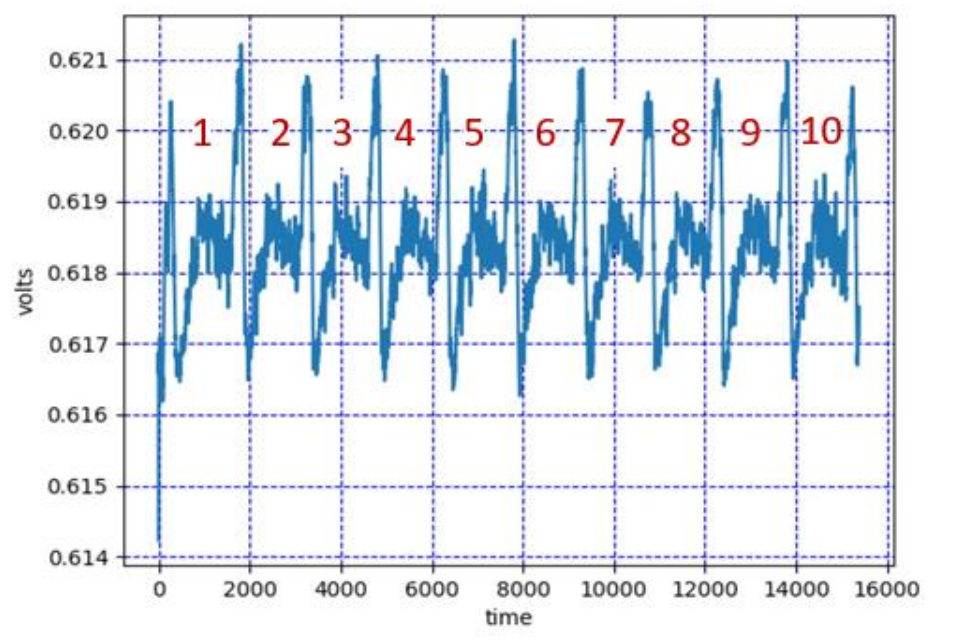
\includegraphics[width=\linewidth]{main thing/Pictures/AES_SPA_trace.png}
            \captionof{figure}{\small An SPA trace revealing the 10 rounds of an AES encryption.}
        \end{minipage}
    \end{figure}
\end{frame}


\begin{frame}
    \frametitle{Averaging Traces to Reduce Noise}

    The electrical signals measured are very small and inherently noisy. The random electronic noise component can obscure the underlying patterns.
    
    To improve the clarity of the trace for visual inspection, an attacker can capture multiple traces of the same operation and \textbf{compute their average}.
    
    \begin{alertblock}{}
         Since the electronic noise is typically \textbf{normally distributed} with a mean of zero, \textbf{averaging causes the noise to cancel out}. \newline
         The underlying deterministic signal, which is consistent across traces, is reinforced.
    \end{alertblock}
    
    This technique significantly improves the signal-to-noise ratio (SNR) for visual analysis.
\end{frame}

\begin{frame}
    \frametitle{Interpreting SPA Traces}

    By visually inspecting a power trace, an attacker can identify large-scale features of the cryptographic algorithm.
    
    \begin{itemize}
        \item \textbf{Algorithmic Rounds:} Iterative ciphers like DES and AES produce repetitive patterns, where each repetition corresponds to one round of the algorithm.
        \item \textbf{Distinct Operations:} Different operations within a round, such as substitutions (S-boxes) and permutations (MixColumns), can consume different amounts of power and time, making them distinguishable in the trace.
    \end{itemize}

    This allows an attacker to map the power trace to the known structure of the cryptographic algorithm.
\end{frame}

\begin{frame}
    \begin{figure}
        \centering
        \begin{minipage}{0.48\textwidth}
            \centering
            % Replace with the path to your detailed AES trace image
            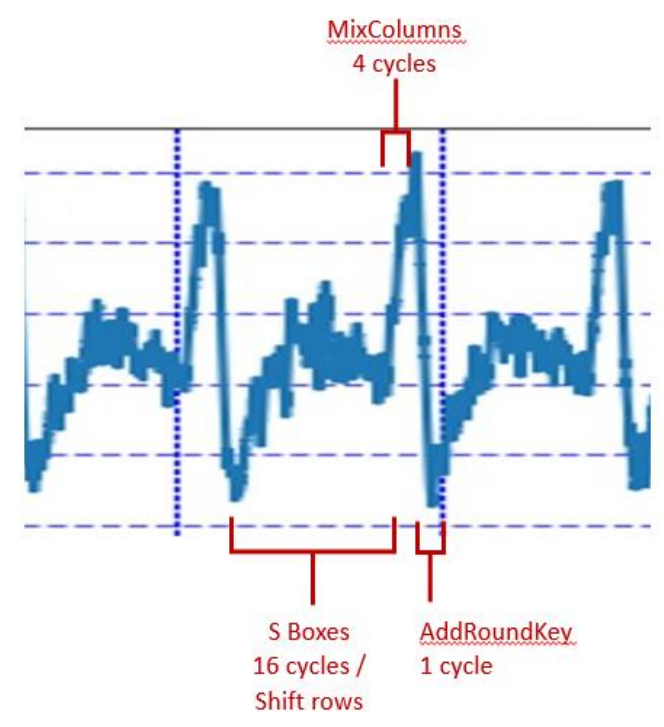
\includegraphics[width=\linewidth]{main thing/Pictures/detailed_AES_SPA_trace.png}
            \captionof{figure}{\small A detailed view of an AES round.}
        \end{minipage}\hfill
        \begin{minipage}{0.48\textwidth}
            \centering
            % Replace with the path to your AES block diagram image
            \includegraphics[width=\linewidth]{path/to/your/AES_diagram.png}
            \captionof{figure}{\small The standard block diagram of an AES round for comparison.}
        \end{minipage}
    \end{figure}
\end{frame}


\begin{frame}
    \frametitle{Classic SPA Attack: RSA Exponentiation}
    
    A classic example of SPA is the attack on RSA implementations that use the \textbf{square-and-multiply} algorithm for modular exponentiation.

    \begin{itemize}
        \item The algorithm processes the private key one bit at a time.
        \item If the key bit is a '1', it performs a \textbf{square} operation followed by a \textbf{multiply} operation.
        \item If the key bit is a '0', it performs \textbf{only a square} operation.
    \end{itemize}
    
    The additional 'multiply' operation for a '1' bit consumes a different amount of power and takes a different amount of time, creating a distinct and easily recognizable pattern in the power trace.
\end{frame}


\begin{frame}
    \frametitle{Visualizing the RSA Attack}
    
    By observing the sequence of power consumption patterns, an attacker can directly read the bits of the private exponent from the trace.

    \begin{figure}
        \centering
        % Replace with the path to your RSA trace image
        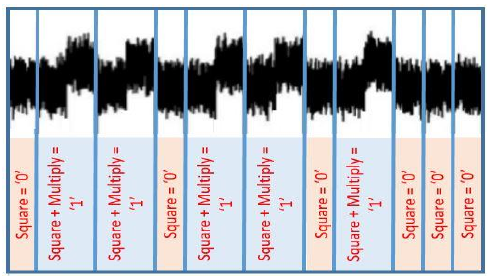
\includegraphics[width=0.8\linewidth]{main thing/Pictures/rsa_exponent.png}
        \captionof{figure}{\small A power trace of an RSA exponentiation. The distinct patterns for 'square' and 'square-and-multiply' operations reveal the secret key bits.}
    \end{figure}

  
\end{frame}